\documentclass[10pt,conference]{IEEEtran}
\IEEEoverridecommandlockouts

% ── Font Setup ───────────────────────────────────────────────────────────────
\usepackage{times}
\usepackage{courier}

% ── Core Packages ────────────────────────────────────────────────────────────
\usepackage[T1]{fontenc}
\usepackage[utf8]{inputenc}
\usepackage[final]{microtype}
\tolerance=1200
\emergencystretch=1.5em
\hyphenpenalty=50
\usepackage{amsmath}
\usepackage{graphicx}
\usepackage{booktabs}
\usepackage{array}
\usepackage{xcolor}
\usepackage[hyphens]{url}
\usepackage{hyperref}
\usepackage{listings}
\usepackage{caption}
\usepackage{float}
\makeatletter
\DeclareTextFontCommand{\texttt}{\ttfamily\hyphenchar\font=-1}
\makeatother

\graphicspath{{figures/}{figures/pingpong/}{figures/ablation/}}

\hypersetup{
  colorlinks=true,
  linkcolor=black,
  citecolor=black,
  urlcolor=black!70
}

% ── Float Spacing Optimization ────────────────────────────────────────────────
\setlength{\floatsep}{5pt plus 2pt minus 2pt}
\setlength{\textfloatsep}{7pt plus 2pt minus 2pt}
\setlength{\intextsep}{5pt plus 2pt minus 2pt}
\setlength{\dblfloatsep}{5pt plus 2pt minus 2pt}
\setlength{\dbltextfloatsep}{7pt plus 2pt minus 2pt}

% ── Code Listing Style ────────────────────────────────────────────────────────
\definecolor{codebg}{gray}{0.96}
\definecolor{coderule}{gray}{0.70}
\definecolor{codecomment}{rgb}{0.35,0.35,0.35}
\definecolor{codekeyword}{rgb}{0.00,0.00,0.52}
\definecolor{codestring}{rgb}{0.45,0.00,0.00}

\lstdefinestyle{ieeestyle}{
  basicstyle=\fontfamily{pcr}\selectfont\fontsize{7.0}{8.5}\selectfont,
  breaklines=true,
  breakatwhitespace=true,
  columns=flexible,
  keepspaces=true,
  frame=tb,
  framesep=3pt,
  rulecolor=\color{coderule},
  backgroundcolor=\color{codebg},
  xleftmargin=4pt,
  xrightmargin=4pt,
  aboveskip=4pt,
  belowskip=4pt,
  keywordstyle=\bfseries\color{codekeyword},
  commentstyle=\itshape\color{codecomment},
  stringstyle=\color{codestring},
  showstringspaces=false,
  numbers=none,
}
\lstset{style=ieeestyle}

% ── Column types ──────────────────────────────────────────────────────────────
\newcolumntype{C}[1]{>{\centering\arraybackslash}p{#1}}
\newcolumntype{L}[1]{>{\raggedright\arraybackslash}p{#1}}

% ── Caption style ────────────────────────────────────────────────────────────
\captionsetup{
  font={small},
  labelfont={bf,small},
  textfont={small},
  labelsep=period,
  justification=justified,
  singlelinecheck=false
}
\captionsetup[table]{
  position=top,
  font={small},
  labelfont={sc,small},
  textfont={small},
  labelsep=newline
}

\urlstyle{same}

% ─────────────────────────────────────────────────────────────────────────────
\begin{document}

\title{Shared-Memory SPSC IPC and io\_uring Wakeup Modes:\\
A Measurement Study of Wakeup Mechanisms and Measurement Controls}

\author{
  \IEEEauthorblockN{%
    \begin{tabular}{@{}c@{\hspace{3em}}c@{\hspace{3em}}c@{}}
      Rahul Raman & Yuvraj Deshmukh & B. Thangaraju
    \end{tabular}}
  \IEEEauthorblockA{
    \textit{Department of Computer Science and Engineering}\\
    \textit{International Institute of Information Technology Bangalore (IIITB)}, Bangalore, India\\
    \begin{tabular}{@{}c@{\hspace{2em}}c@{\hspace{2em}}c@{}}
      rahul.raman@iiitb.ac.in & yuvraj.deshmukh@iiitb.ac.in & b.thangaraju@iiitb.ac.in
    \end{tabular}
  }
}

\maketitle

% ─────────────────────────────────────────────────────────────────────────────
\begin{abstract}
Inter-Process Communication (IPC) performance is a foundational bottleneck in
concurrent, multi-process software systems. Traditional kernel-mediated
mechanisms---POSIX Pipes, UNIX Domain Sockets, POSIX Message Queues---impose
mandatory system calls, context switches, and user-to-kernel memory copying on
every message, creating an irreducible per-message overhead of several
microseconds. Modern high-performance systems reduce this cost by employing
lock-free Single-Producer Single-Consumer (SPSC) shared-memory ring buffers
that transfer payload data entirely in userspace via memcpy into POSIX
shared memory regions. A critical and largely unanswered question, however,
is: when the shared ring empties and the consumer must sleep, which
wakeup primitive should be used---and what does Linux's
io\_uring framework specifically contribute over simpler
alternatives such as futex or eventfd?

This paper presents a rigorous empirical measurement study that decouples
payload transport from wakeup-mechanism signaling and applies a two-suite
evaluation framework: (1) a wakeup-mechanism ablation comparing six
coordination strategies (busy\_poll, spin\_backoff,
adaptive, futex, eventfd, io\_uring) on an
identical cache-aligned SPSC ring under saturated and bursty traffic
conditions across a 64\,B--1\,MiB message-size sweep; and (2) a
corrected depth-1 ping-pong latency suite in which both the send and
receive timestamps are recorded on the single initiator core using
CLOCK\_MONOTONIC\_RAW, eliminating cross-core TSC drift and
in-flight pipelining artefacts, reporting full percentile distributions
(P50, P90, P99, P99.9) over 100\,000 round-trips per configuration.

Our results show that the shared-memory ring delivers the primary performance
gains. Spinning variants achieve median single-trip latencies of
345--381\,ns at 64\,B---over a 15$\times$ improvement over pipe or
socket---and peak direct-ring streaming throughput of 28.17\,GiB/s at 64\,KiB.
In depth-1 ping-pong tests (Suite 2), io\_uring incurs a modest per-event
ring submission overhead (+2.8\,$\mu$s over futex at 64\,B).
However, under bursty wakeup conditions (Suite 1), where wakeups occur when the
ring empties, io\_uring performs on par with futex and
eventfd ($\approx$1.09--1.10\,ms median wakeup latency with
$\approx$0\,\% idle CPU consumption).
The shared-memory ring, rather than the wakeup primitive, delivers the primary
gain.  A frequency-pinned replication (\texttt{performance} governor and
\texttt{no\_turbo=1}) reproduces the close ordering of the kernel-sleeping
variants.  We additionally evaluate SQPOLL as a separate configuration:
its 64\,B bursty wakeup median (1058.5\,$\mu$s) is close to interrupt-mode
io\_uring (1095.0\,$\mu$s), rather than a decisive improvement.
\end{abstract}

\begin{IEEEkeywords}
io\_uring, IPC, shared memory, SPSC ring buffer, lock-free, wakeup mechanism,
latency, throughput, Linux kernel, systems performance
\end{IEEEkeywords}

% ─────────────────────────────────────────────────────────────────────────────
\section{Introduction}

Modern software infrastructure---spanning high-frequency trading (HFT) matching
engines, real-time database kernels, media processing pipelines, and
containerised microservice mesh proxies---relies heavily on efficient
Inter-Process Communication.  Even a modest per-message overhead of a few
microseconds accumulates to tens of milliseconds when millions of messages flow
per second.  At 10\,Mop/s, a 3\,$\mu$s per-message syscall overhead alone
consumes 30\,\% of the CPU budget.

Linux provides a rich set of mature IPC primitives.  POSIX FIFOs and UNIX
domain sockets route all data through the kernel, imposing context switches and
double memory copies on every message.  POSIX message queues add priority
ordering but retain kernel-mediated delivery semantics.  Shared memory avoids
the data-copy penalty by mapping identical physical pages into both producer and
consumer address spaces; the kernel is contacted only for initial setup.

The cost of these kernel interactions is non-trivial and grows with message
rate.  A \texttt{write}/\texttt{read} pair on a POSIX pipe costs approximately
1--3\ $\mu$s in system-call overhead on modern Linux, independent of payload
size.  For a system exchanging 5\,Mmsg/s, this overhead alone consumes a full
CPU core.  Beyond raw syscall cost, kernel buffers are allocated from a
different NUMA domain relative to the application heap on multi-socket machines,
adding DRAM access latency to every message.  Real-time systems with sub-1\,ms
SLAs cannot tolerate this overhead when message rates exceed a few hundred
thousand per second.

Lock-free SPSC ring buffers---popularised by the LMAX
Disruptor~\cite{disruptor} and Intel DPDK~\cite{dpdk}---take shared memory a
step further by coordinating access using only atomic load/store instructions on
cache-line-aligned indices, avoiding any kernel involvement on the data path.
Message delivery in the uncontended case reduces to a \texttt{memcpy} plus two
atomic index updates, costing roughly 200\,ns at 64\,B---an order of magnitude
below any kernel-mediated mechanism.

A remaining challenge is the \emph{empty-ring wakeup problem}: when the ring is
empty, busy-spinning wastes a full CPU core; sleeping the consumer requires a
kernel-level wakeup mechanism.

Linux's \texttt{io\_uring} interface (introduced in kernel 5.1~\cite{axboe2019})
has attracted substantial interest for its promise of zero-syscall I/O.  A
growing body of practitioner literature presents ``\texttt{io\_uring}-based IPC
rings'' as offering superior latency and throughput over both traditional IPC
and simpler shared-memory approaches.  However, these claims conflate two
independent design decisions: (1)~the payload data path choice (shared memory
vs.\ kernel-copy), and (2)~the wakeup mechanism choice (\texttt{io\_uring}
vs.\ \texttt{futex} vs.\ spin).  No prior measurement study isolates these
dimensions on identical hardware with a controlled ablation.

\subsection*{Contributions}

\begin{enumerate}
  \item \textbf{Controlled wakeup ablation.}  Six pluggable wakeup strategies
        are implemented on a bit-identical SPSC ring buffer; their impact on
        latency, throughput, CPU utilization, and syscall rate is measured
        across a 64\,B--1\,MiB payload sweep.

  \item \textbf{Corrected depth-1 ping-pong protocol.}  Queue depth is
        enforced at~1 and both round-trip endpoints are timestamped on the
        same core with \texttt{CLOCK\_MONOTONIC\_RAW}, eliminating TSC skew
        and pipelining artefacts.

  \item \textbf{Tail-latency characterisation.}  P50, P90, P99, P99.9, and
        95\,\% confidence intervals are reported for every supported payload
        size, including 64\,KiB (10\,000 rounds) and 1\,MiB (2\,000 rounds).
        The 64\,B and 4\,KiB configurations use 100\,000 and 50\,000 rounds,
        respectively.

  \item \textbf{Explicit measurement scope.}  We report interrupt-mode and
        SQPOLL io\_uring as distinct configurations, and record fixed-frequency
        settings for the low-load wakeup measurements.

  \item \textbf{Reproducible artifact.}  All source code, raw CSV data, and
        figure-generation scripts are published at
        \url{https://github.com/Rahul09123/io_uring-IPC}.
\end{enumerate}

% ─────────────────────────────────────────────────────────────────────────────
\section{Background \& Related Work}

\subsection{Traditional Kernel-Mediated IPC}

\textbf{POSIX Pipes (FIFOs)} (Stevens and Rago~\cite{stevens2013}) provide uni-directional byte streams backed by a
kernel circular buffer (default 64\,KiB, tunable to 1\,MiB via
\texttt{fcntl(F\_SETPIPE\_SZ)}).  Every \texttt{write} copies data from user
to kernel space; every \texttt{read} copies it back.  The producer and consumer
alternate between running and sleeping states as the pipe buffer fills and
drains, incurring scheduler-wakeup latency on each transition.  At very small
messages (64\,B), the pipe's fixed per-syscall entry cost dominates; at large
messages ($\geq$256\,KiB), buffer-saturation and block-layer flushing limit
throughput to $\approx$5--6\,GiB/s regardless of CPU speed.

\textbf{UNIX Domain Sockets} bypass the network stack but retain the socket
buffer abstraction (\texttt{sk\_buff}).  Each \texttt{sendmsg}/\texttt{recvmsg}
pair requires a system call and a socket-layer serialisation lock
(\texttt{mutex\_lock} visible in flamegraph traces).  Socket send/receive
buffers are tuned to 2\,MiB via \texttt{SO\_SNDBUF}/\texttt{SO\_RCVBUF} in
our implementation.  Despite the per-call overhead, UNIX sockets achieve
competitive throughput at large payload sizes because the kernel socket buffer
is not bounded by a fixed slot count and can leverage zero-copy page-flipping
for contiguous large writes.

\textbf{POSIX Message Queues (\texttt{mqueue})} deliver structured,
priority-sorted messages via a virtual filesystem inode under
\texttt{/dev/mqueue}.  A key optimisation---\texttt{pipelined\_send}---delivers
directly into a blocked receiver's address space when one is already waiting,
bypassing intermediate queue staging and making \texttt{mqueue} competitive
with shared-memory rings at small message sizes.  However, the default maximum
message size is 8\,KiB and the maximum queue depth is 10 messages, both
controlled by kernel tunables (\texttt{fs.mqueue.msgsize\_max},
\texttt{fs.mqueue.msg\_max}), imposing hard architectural limits at scale.

\begin{table}[H]
  \centering
  \caption{Kernel-IPC System-Call and Copy Costs per Message}
  \label{tab:ipc_cost}
  \small
  \begin{tabular}{@{}L{1.8cm}L{1.5cm}L{1.5cm}L{2.5cm}@{}}
    \toprule
    \textbf{Mechanism} & \textbf{Syscalls /msg} & \textbf{Copies /msg} & \textbf{Kernel buffer} \\
    \midrule
    POSIX Pipe   & 2 & 2 & Ring buf (64\,KiB--1\,MiB) \\
    UNIX Socket  & 2 & 2 & \texttt{sk\_buff} (up to 2\,MiB) \\
    POSIX MQ     & 2 & 1--2 & VFS inode (10 msgs) \\
    SHM Ring     & 0 & 1 & None (userspace) \\
    \bottomrule
  \end{tabular}
\end{table}

\subsection{Lock-Free SPSC Shared-Memory Rings}

Shared-memory IPC maps identical physical pages into producer and consumer
address spaces via \texttt{shm\_open} and \texttt{mmap}.  SPSC ring buffers
(Lamport~\cite{lamport1983}, Herlihy and Shavit~\cite{herlihy2008}, LMAX Disruptor~\cite{disruptor}, DPDK
\texttt{rte\_ring}~\cite{dpdk}) coordinate using a pair of atomic integer
indices.  The critical correctness rule is: the producer advances \texttt{head}
with \texttt{release} ordering after writing payload; the consumer reads
\texttt{head} with \texttt{acquire} ordering before consuming.

The C++17 memory model formally defines these orderings.  A \emph{release
store} ensures all prior writes are visible to any thread that subsequently
performs an \emph{acquire load} of the same variable.  For an SPSC ring, this
means the consumer observing \texttt{head~>~tail} is guaranteed to see the
complete payload written by the producer before \texttt{head} was advanced.
Using \texttt{memory\_order\_relaxed} on \texttt{head} (a common optimisation)
works on x86 due to Total Store Order (TSO) but is technically undefined
behaviour on weakly-ordered architectures (ARM, RISC-V, Power) that permit
Store-Load reordering.  We use \texttt{memory\_order\_seq\_cst} on the
publish store to maintain portability and prevent the lost-wakeup race.

\textbf{False sharing}---where producer and consumer cache lines collide---is
prevented by placing \texttt{head}, \texttt{tail}, and control flags on
separate 64-byte-aligned cache lines using \texttt{alignas(64)}.  Without this
separation, a producer store to \texttt{head} invalidates the cache line
containing \texttt{tail} on the consumer core, forcing a cache-coherency
RFO (Request For Ownership) on every slot exchange and doubling effective
memory latency.

\subsection{The io\_uring Interface}

Introduced by Jens Axboe~\cite{axboe2019} and merged in Linux~5.1,
\texttt{io\_uring} exposes two ring buffers shared between userspace and the
kernel: the Submission Queue (SQ) and the Completion Queue (CQ).  In the
default interrupt-driven mode (\texttt{flags=0}), a single
\texttt{io\_uring\_enter} system call submits all pending SQEs and optionally
waits for completions.  In SQPOLL mode (\texttt{IORING\_SETUP\_SQPOLL}), a
dedicated kernel poller thread eliminates the syscall entirely but requires
elevated privileges.

In our implementation, \texttt{io\_uring} is used \emph{exclusively for the
wakeup signaling path}.  When the consumer sleeps, it submits an
\texttt{IORING\_OP\_READ} on a named FIFO and blocks in
\texttt{io\_uring\_submit\_and\_wait}.  When the producer detects
\texttt{consumer\_sleeping}~=~1, it submits an \texttt{IORING\_OP\_WRITE} to
the same FIFO.  The payload data path is pure \texttt{memcpy} into shared
memory---\texttt{io\_uring} never touches message bytes.

\subsection{Prior Work on io\_uring Performance}

Didona et~al.~\cite{didona2022} compared \texttt{libaio}, SPDK, and
\texttt{io\_uring} for storage I/O, demonstrating that polling makes \texttt{io\_uring}
competitive with SPDK for sequential workloads.  Ren and Trivedi~\cite{ren2023} demonstrated
that \texttt{io\_uring} can match kernel-bypass performance for certain NVMe
access patterns.  Neither study addresses the question of wakeup-primitive
selection for shared-memory IPC, leaving this dimension unexplored.  Our work
fills this gap with a controlled ablation study on a single fixed ring design.

% ─────────────────────────────────────────────────────────────────────────────
\section{System Design}

Our architecture cleanly separates the data path from the control path.

\subsection{Lock-Free SPSC Ring Buffer Layout}

The shared ring buffer is a single POSIX shared memory object opened via
\texttt{shm\_open} and mapped with \texttt{mmap} into both the producer and
consumer address spaces.

\begin{lstlisting}[language=C++,caption={Cache-aligned SPSC RingBuffer (common.h)}]
struct alignas(64) RingBuffer {
  alignas(64) atomic<uint64_t> head;   // Producer write index
  alignas(64) atomic<uint64_t> tail;   // Consumer read index
  alignas(64) atomic<uint32_t> consumer_sleeping;

  struct alignas(64) Slot {
    uint64_t send_ns;           // Producer timestamp (CLOCK_MONOTONIC_RAW)
    uint64_t wakeup_publish_ns; // Wakeup-signal timestamp
    uint32_t size;              // Payload bytes written
    char     data[MAX_PAYLOAD]; // Up to 1 MiB of payload
  };
  Slot slots[NUM_SLOTS];        // Fixed 64-slot ring (~64 MiB total)
};
\end{lstlisting}

Three design properties are critical.

\textbf{(1) Cache-line isolation.}  \texttt{head}, \texttt{tail}, and
\texttt{consumer\-\_sleeping} each occupy their own 64-byte cache line.
Without this separation, a producer write to \texttt{head} invalidates
the cache line containing \texttt{tail} on the consumer core, forcing
an RFO (Request For Ownership) round-trip on every slot transition.  Our
hardware counter data (Table~\ref{tab:cache}) confirms this: the SHM
Ring's 4.97\,\% LLC miss rate compares favourably to 30--34\,\% for
mechanisms that traverse kernel buffers and inadvertently evict ring
control variables.

\textbf{(2) Sequential consistency at publish boundaries.}
\texttt{head} is stored with \texttt{memory\-\_order\-\_seq\-\_cst}
to prevent Store-Load reordering that could cause the producer to read
stale \texttt{consumer\-\_sleeping~=~0} and skip sending a wakeup,
silently deadlocking the consumer.  On x86 (TSO), this is equivalent to
a plain store followed by a \texttt{mfence}; on ARM64 it compiles to a
\texttt{stlr} (store-release) instruction.

\textbf{(3) Lost-wakeup prevention.}  A classic race exists in any
producer-consumer pair: the consumer checks \texttt{head == tail}
(empty), decides to sleep, but before setting
\texttt{consumer\-\_sleeping}, the producer writes a slot and checks
\texttt{consumer\-\_sleeping~=~0} (decides not to signal), then the
consumer sets \texttt{consumer\-\_sleeping~=~1} and waits---forever.
We eliminate this race by having the consumer set
\texttt{consumer\-\_sleeping~=~1} \emph{first}, then re-check
\texttt{head~!=~tail} under a full memory fence.  If a slot arrived in
the window, the re-check catches it and the consumer proceeds without
sleeping.

\textbf{Data-flow walkthrough.}  On every message transfer: (a)~the producer
calls \texttt{memcpy} into \texttt{slots[head \% NUM\_SLOTS].data}, writes the
timestamp and size, then executes a seq\_cst store to \texttt{head};
(b)~the consumer spin-reads \texttt{head} with acquire ordering; once it
observes \texttt{head > tail}, it processes the slot and advances \texttt{tail}
with a release store; (c)~if the consumer finds the ring empty after its
deadlock-prevention recheck, it invokes the configured wakeup primitive to
sleep.  Steps (a) and (b) involve zero system calls; step (c) invokes at most
one system call per wakeup event.

\subsection{Pluggable Wakeup Layer: Six Ablation Variants}

To isolate the contribution of the wakeup mechanism, we implement six
interchangeable wakeup modules on a single, bit-identical SPSC ring buffer data
structure.  Each primitive is invoked via its standard Linux kernel system
interface (Linux man-pages~\cite{linux-man}): Only the
functions \texttt{consumer\_wait()} and \texttt{producer\_signal()} differ,
guaranteeing that any observed latency difference is attributable solely to
the wakeup mechanism.

\paragraph{1.~\texttt{busy\_poll}.}
The consumer spins in a tight \texttt{while(head.load(relaxed) == tail)} loop
with no backoff.  Zero system calls are issued.  Latency is minimal
($\approx$200\,ns) but one CPU core is permanently pegged at 100\,\%.

\paragraph{2.~\texttt{spin\_backoff}.}
Same tight spin with an \texttt{\_mm\_pause()} intrinsic on every iteration.
\texttt{\_mm\_pause} inserts a brief pipeline delay on x86, reducing
memory-ordering storms and lowering power by $\approx$20\,\% vs.\
\texttt{busy\_poll} with negligible latency impact.

\paragraph{3.~\texttt{adaptive}.}
The consumer spins for up to 500 iterations; if no data arrives, it falls back
to a \texttt{futex} sleep.  This hybrid targets low-latency workloads where the
ring is rarely empty (spin wins) while gracefully handling burst-idle traffic
(futex sleep saves power).

\paragraph{4.~\texttt{futex}.}
The consumer stores~1 to \texttt{consumer\-\_sleeping} and calls
\texttt{SYS\-\_futex(FUTEX\-\_WAIT)}.  The kernel checks the address
atomically; if it still reads~1, the thread is suspended.  The producer
stores~0 and calls \texttt{FUTEX\-\_WAKE}.  One system call per sleep
and per wakeup event.

\paragraph{5.~\texttt{eventfd}.}
The consumer \texttt{poll}s an eventfd file descriptor and then \texttt{read}s
to consume the wakeup token.  The producer \texttt{write}s~1 to the eventfd.
The eventfd is compatible with \texttt{epoll}/\texttt{select}, easing
integration into existing event-loop frameworks.

\paragraph{6.~\texttt{io\_uring}.}
The consumer submits an \texttt{IORING\-\_OP\-\_READ} SQE targeting a
named FIFO (\texttt{/tmp/\allowbreak uring\-\_sig\-\_fifo}) and blocks
in \texttt{io\-\_uring\-\_submit\-\_and\-\_wait\-(ring,~1)}.  The
producer submits an \texttt{IORING\-\_OP\-\_WRITE} SQE to the same FIFO
and calls \texttt{io\-\_uring\-\_submit}.  The \texttt{io\-\_uring}
context can simultaneously monitor additional FDs, making it advantageous
for frameworks managing many concurrent channels.  Our primary ablation evaluates
standard interrupt mode (\texttt{flags=0}); additionally, the implementation provides
runtime support for \texttt{IORING\_SETUP\_SQPOLL} (SQPOLL mode via \texttt{USE\_SQPOLL=1}),
which offloads ring polling to an asynchronous kernel thread under \texttt{CAP\_SYS\_ADMIN}.

\begin{table}[H]
  \centering
  \caption{Wakeup Mechanism Properties Summary}
  \label{tab:wakeup}
  \small
  \begin{tabular}{@{}L{1.8cm}lcc@{}}
    \toprule
    \textbf{Variant} & \textbf{Wait Strategy} & \textbf{Idle CPU} & \textbf{Sys/wake}\\
    \midrule
    \texttt{busy\_poll}    & Tight spin         & 100\,\%        & 0   \\
    \texttt{spin\_back.}   & Spin+PAUSE         & High           & 0   \\
    \texttt{adaptive}      & Spin-then-futex    & Low            & 0--1 \\
    \texttt{futex}         & FUTEX\_WAIT        & {$\approx$}0\,\% & 2 \\
    \texttt{eventfd}       & poll+read          & {$\approx$}0\,\% & 2 \\
    \texttt{io\_uring}     & sub.\_and\_wait    & {$\approx$}0\,\% & 2 \\
    \bottomrule
  \end{tabular}
\end{table}

% ─────────────────────────────────────────────────────────────────────────────
\section{Experimental Methodology}

\subsection{Two-Suite Benchmark Framework}

\textbf{Suite 1 --- Wakeup-Mechanism Ablation.}
The producer streams messages continuously under two regimes:
\emph{saturated} (back-to-back sends; ring rarely empties) and
\emph{bursty} (64-message burst, then 1\,ms sleep; ring empties every burst).
The bursty regime directly exposes wakeup primitive latency.  Payload sizes
sweep across $\{$64\,B, 256\,B, 1\,KiB, 4\,KiB, 64\,KiB, 1\,MiB$\}$.
$N=15$ measured runs per configuration (one warmup discarded).

\textbf{Suite 2 --- Corrected Depth-1 Ping-Pong.}
Queue depth is strictly enforced to~1: the initiator sends one message and
blocks waiting for the echo server to reflect it before sending the next.
Both $t_{\text{start}}$ and $t_{\text{end}}$ are recorded on
\textbf{Initiator Core~1} using
\texttt{clock\_gettime(CLOCK\_MONOTONIC\_RAW)}.  Single-trip latency:
\[
  L_{\text{trip}} = \frac{t_{\text{end}} - t_{\text{start}}}{2} \quad [\mu\text{s}]
\]
100\,000 round-trips per configuration; 1\,000 warmup trips discarded.
P50, P90, P99, and P99.9 percentiles reported.

\subsection{Hardware and System Configuration}

\begin{table}[H]
  \centering
  \caption{Reference Test Environment}
  \label{tab:env}
  \small
  \begin{tabular}{@{}L{3.0cm}L{4.8cm}@{}}
    \toprule
    \textbf{Parameter} & \textbf{Value}\\
    \midrule
    System          & ASUS Vivobook K3605ZF \\
    OS              & Ubuntu 24.04.4 LTS (kernel 6.x) \\
    CPU             & Intel Core i5-12500H (Alder Lake, 12th Gen) \\
    Architecture    & Hybrid P/E-core \\
    Cores/Threads   & 12 Physical / 16 Logical \\
    Frequency       & 400--4500\,MHz (boost) \\
    L1d Cache       & 448\,KiB (12 instances) \\
    L2 Cache        & 9\,MiB (6 instances) \\
    L3 Cache        & 18\,MiB (shared) \\
    RAM             & 16\,GiB DDR4-3200 \\
    Storage         & 512\,GB Samsung NVMe SSD \\
    Compiler        & g++ -O2, C++17 \\
    liburing        & System package, Ubuntu 24.04 \\
    CPU Governor    & \texttt{performance}; \texttt{intel\_pstate.no\_turbo=1} \\
    \bottomrule
  \end{tabular}
\end{table}

\textbf{Core affinity.}  Producer/Initiator pinned to Core~1; Consumer/
Echo-Server pinned to Core~2 via \texttt{sched\_setaffinity}.  Both cores
share the 18\,MiB L3 cache, keeping the ring buffer warm across the
inter-process boundary.

\textbf{CPU tuning and frequency-pinned replication.}  The final ablation and
ping-pong runs were collected on the native Linux host with Core~1 and Core~2
pinned, the \texttt{performance} governor on both cores, and
\texttt{intel\_pstate.no\_turbo=1}.  These settings are recorded in
\texttt{data/environment\_ablation.txt} and
\texttt{data/environment\_pingpong.txt}.  Core isolation through
\texttt{isolcpus}/\texttt{nohz\_full} was not used; residual scheduler and
idle-state effects therefore remain a limitation.

\subsection{Statistical Methodology}

For each (mechanism, payload size) pair we compute:
\begin{align*}
  \bar{T} &= \frac{1}{N}\sum_{k=1}^{N} T_k \;\;[\text{GiB/s}], \quad
  \bar{L} = \frac{1}{M}\sum_{i=1}^{M} L_i \;\;[\mu\text{s}] \\
  \sigma_L &= \sqrt{\frac{1}{M}\sum_{i=1}^{M} (L_i - \bar{L})^2}
\end{align*}
where $N=15$ is the run count and $M$ is messages per run.  95\,\% confidence
intervals use the Student-$t$ approximation on run-level means.

\subsection{Workload Volumes}

\begin{table}[H]
  \centering
  \caption{Workload Volumes per (Mechanism, Size) Configuration}
  \label{tab:volumes}
  \small
  \begin{tabular}{@{}L{2.4cm}L{1.7cm}L{1.7cm}L{1.7cm}@{}}
    \toprule
    \textbf{Mechanism} & \textbf{$\leq$1\,KiB} & \textbf{4--64\,KiB} & \textbf{$\geq$256\,KiB} \\
    \midrule
    POSIX Pipe   & 32\,MiB  & 256\,MiB & 2\,GiB \\
    POSIX MQ     & 32\,MiB  & 256\,MiB & 2\,GiB \\
    UNIX Socket  & 2\,GiB   & 2\,GiB   & 2\,GiB \\
    SHM Ring     & 2\,GiB   & 2\,GiB   & 2\,GiB \\
    \bottomrule
  \end{tabular}
\end{table}

% ─────────────────────────────────────────────────────────────────────────────
\section{Empirical Results}

\subsection{Unloaded Ping-Pong Latency (Suite 2)}

Table~\ref{tab:pingpong} reports single-trip latency distributions (P50, P90, P99, P99.9, and mean $\pm$ 95\% CI) at all four message sizes. Values are drawn consistently from the root \texttt{data/pingpong\_*\_summary.csv} files; legacy duplicates and the conflicting aggregate file are not used.

\begin{table}[H]
  \centering
  \caption{Single-Trip Ping-Pong Latency Distributions ($\mu$s). Each row reports P50, P90, P99, P99.9, and mean $\pm$ 95\% CI from the canonical root summary CSVs.}
  \label{tab:pingpong}
  \resizebox{\columnwidth}{!}{%
  \small
  \begin{tabular}{@{}lrrrrr@{}}
    \toprule
    \textbf{Transport / Variant} & \textbf{P50} & \textbf{P90} & \textbf{P99} & \textbf{P99.9} & \textbf{Mean $\pm$ CI} \\
    \midrule
    \multicolumn{6}{@{}l}{\emph{Message Size: 64\,B --- lower is better}} \\[1pt]
    \texttt{shm (adaptive)}   & \textbf{0.345} & 0.439 & 0.505 & 1.189 & 0.363 $\pm$ 0.002 \\
    \texttt{shm (busy\_poll)} & 0.381          & 0.500 & 0.851 & 1.584 & 0.414 $\pm$ 0.003 \\
    \texttt{shm (spin\_back)} & 0.727          & 1.284 & 1.317 & 1.823 & 0.846 $\pm$ 0.002 \\
    \texttt{shm (futex)}      & 5.001          & 5.097 & 6.395 & 8.872 & 5.033 $\pm$ 0.002 \\
    \texttt{shm (eventfd)}    & 5.039          & 5.169 & 6.444 & 8.832 & 5.081 $\pm$ 0.002 \\
    \texttt{pipe}             & 5.290          & 5.400 & 7.016 & 10.984 & 5.345 $\pm$ 0.005 \\
    \texttt{posix\_mq}        & 5.567          & 5.685 & 7.361 & 9.824 & 5.629 $\pm$ 0.002 \\
    \texttt{unix\_socket}     & 5.496          & 7.214 & 8.196 & 11.330 & 5.900 $\pm$ 0.017 \\
    \texttt{shm (io\_uring)}  & 8.150          & 8.426 & 10.351 & 14.347 & 8.236 $\pm$ 0.003 \\
    \midrule
    \multicolumn{6}{@{}l}{\emph{Message Size: 4\,KiB --- lower is better}} \\[1pt]
    \texttt{shm (adaptive)}   & \textbf{2.263} & 2.339 & 2.422 & 5.072 & 2.271 $\pm$ 0.001 \\
    \texttt{shm (busy\_poll)} & 2.306          & 2.413 & 3.576 & 8.527 & 2.353 $\pm$ 0.004 \\
    \texttt{shm (spin\_back)} & 2.663          & 2.724 & 3.120 & 5.494 & 2.656 $\pm$ 0.002 \\
    \texttt{shm (futex)}      & 6.735          & 6.899 & 8.575 & 10.677 & 6.808 $\pm$ 0.003 \\
    \texttt{shm (eventfd)}    & 6.809          & 7.137 & 8.403 & 10.874 & 6.898 $\pm$ 0.011 \\
    \texttt{pipe}             & 7.147          & 7.470 & 8.825 & 12.966 & 7.248 $\pm$ 0.004 \\
    \texttt{posix\_mq}        & 8.746          & 9.028 & 10.493 & 13.275 & 8.813 $\pm$ 0.004 \\
    \texttt{shm (io\_uring)}  & 9.855          & 10.119 & 12.056 & 15.679 & 9.923 $\pm$ 0.005 \\
    \texttt{unix\_socket}     & 11.864         & 12.657 & 13.609 & 19.349 & 11.093 $\pm$ 0.016 \\
    \midrule
    \multicolumn{6}{@{}l}{\emph{Message Size: 64\,KiB --- lower is better}} \\[1pt]
    \texttt{shm (busy\_poll)} & \textbf{23.293} & 23.845 & 26.982 & 48.473 & 23.280 $\pm$ 0.038 \\
    \texttt{shm (adaptive)}   & 23.888          & 24.006 & 25.829 & 27.300 & 23.858 $\pm$ 0.013 \\
    \texttt{shm (spin\_back)} & 24.204          & 24.298 & 25.881 & 27.637 & 24.187 $\pm$ 0.015 \\
    \texttt{shm (eventfd)}    & 27.244          & 27.478 & 29.342 & 31.348 & 27.228 $\pm$ 0.014 \\
    \texttt{shm (futex)}      & 27.227          & 27.464 & 29.242 & 31.836 & 27.216 $\pm$ 0.019 \\
    \texttt{unix\_socket}     & 28.284          & 29.270 & 32.880 & 37.986 & 28.362 $\pm$ 0.022 \\
    \texttt{shm (io\_uring)}  & 29.409          & 29.689 & 31.802 & 33.743 & 29.262 $\pm$ 0.019 \\
    \texttt{pipe}             & 35.861          & 36.380 & 40.106 & 41.696 & 35.935 $\pm$ 0.017 \\
    \texttt{posix\_mq}        & 35.869          & 36.721 & 39.651 & 42.714 & 35.988 $\pm$ 0.038 \\
    \midrule
    \multicolumn{6}{@{}l}{\emph{Message Size: 1\,MiB --- lower is better}} \\[1pt]
    \texttt{unix\_socket}     & \textbf{241.094} & 248.331 & 261.743 & 365.375 & 242.922 $\pm$ 0.291 \\
    \texttt{shm (busy\_poll)} & 267.243          & 276.180 & 285.295 & 295.643 & 269.615 $\pm$ 0.205 \\
    \texttt{shm (spin\_back)} & 267.366          & 276.029 & 285.168 & 297.980 & 269.596 $\pm$ 0.203 \\
    \texttt{shm (eventfd)}    & 276.786          & 283.946 & 297.494 & 327.397 & 278.874 $\pm$ 0.316 \\
    \texttt{shm (adaptive)}   & 278.976          & 288.360 & 300.819 & 314.115 & 282.830 $\pm$ 2.696 \\
    \texttt{shm (futex)}      & 278.034          & 286.596 & 296.704 & 335.171 & 280.502 $\pm$ 0.236 \\
    \texttt{shm (io\_uring)}  & 281.154          & 289.455 & 301.202 & 335.805 & 283.185 $\pm$ 0.256 \\
    \texttt{pipe}             & 473.293          & 482.965 & 542.826 & 1429.330 & 479.538 $\pm$ 3.410 \\
    \texttt{posix\_mq}        & N/A              & N/A     & N/A     & N/A     & N/A \\
    \bottomrule
  \end{tabular}}
\end{table}

\textbf{Key observations:}

\textbf{(1) 13.6$\times$ spinning advantage at small messages.}
At 64\,B, \texttt{adaptive} (0.345\,$\mu$s) and \texttt{busy\_poll}
(0.381\,$\mu$s) are over 13$\times$ lower than any kernel-sleeping variant.  This
gap represents scheduler wakeup latency: transitioning a sleeping thread to
running requires dequeueing, CPU selection, and context switching---costing
2--4\,$\mu$s on a loaded Linux system.

\textbf{(2) Kernel-sleeping variants converge regardless of primitive.}
\texttt{futex} (5.001\,$\mu$s), \texttt{eventfd} (5.039\,$\mu$s), and
\texttt{io\_uring} (8.150\,$\mu$s) all converge to 5.0--8.2\,$\mu$s P50 at 64\,B.
The slight elevation of \texttt{io\_uring} reflects SQ/CQ ring entry overhead. (These figures are recomputed from the full 100,000-trip raw distribution underlying Table~\ref{tab:pingpong}; the \texttt{io\_uring} value differs marginally from earlier aggregate-based estimates reported in preliminary analysis.)

\textbf{(3) POSIX MQ is valid through 64\,KiB in the recorded run.}
The repository's 64\,KiB summary records 10,000 round trips (P50 36.668\,$\mu$s).
The 256\,KiB and 1\,MiB rows are explicitly marked unsupported by the host
POSIX-MQ message-size limit and are reported as N/A.

\textbf{(4) UNIX Socket wins at 1\,MiB.}
242.90\,$\mu$s vs.\ 270.9--281.3\,$\mu$s for SHM variants.  The kernel socket
buffer handles large writes via page-flipping, bypassing the fixed-slot
recycling stall that limits the SHM ring.

\subsection{Ablation: Wakeup Variant Comparison (Suite 2)}

At 1\,MiB, all six SHM variants converge near 271--281\,$\mu$s
(Table~\ref{tab:pingpong}). Copying 1\,MiB across the ring
dominates all wakeup mechanism overhead, making wakeup selection irrelevant at
that message size.  Wakeup mechanism matters only when message service time is
short enough to be latency-dominated.

\subsection{Streaming Throughput: Saturated Regime (Suite 1)}

Table~\ref{tab:throughput} presents mean throughput; Figure~\ref{fig:throughput}
visualises the full size sweep.

\begin{table}[H]
  \centering
  \caption{Streaming Throughput (GiB/s) --- Saturated Regime, $N=15$ Runs}
  \label{tab:throughput}
  \small
  \begin{tabular}{@{}L{2.6cm}cccc@{}}
    \toprule
    \textbf{Wakeup Variant} & \textbf{64\,B} & \textbf{4\,KiB} &
        \textbf{64\,KiB} & \textbf{1\,MiB} \\
    \midrule
    \texttt{busy\_poll}    & 0.316 & 10.17 & \textbf{15.75} & \textbf{8.65} \\
    \texttt{spin\_backoff} & \textbf{0.344} & 10.16 & 14.54 & 8.61 \\
    \texttt{adaptive}      & 0.338 & 10.43 & 15.53 & 8.36 \\
    \texttt{eventfd}       & 0.262 & 9.54 & 13.74 & 8.37 \\
    \texttt{futex}         & 0.300 & \textbf{10.68} & 15.60 & 8.18 \\
    \texttt{io\_uring}     & 0.332 & 9.92 & 13.37 & 8.12 \\
    \bottomrule
  \end{tabular}
\end{table}



\textbf{Key observations:}

\textbf{(1) Saturated throughput is primarily data-path bound.}
Under fully saturated load the ring rarely empties, so the wakeup primitive is
rarely invoked.  The six variants remain in the same order of magnitude, with
the refreshed 64\,KiB results spanning 13.37--15.75\,GiB/s.

\textbf{(2) Direct-ring baseline remains faster than the pipe baseline.}
The separately measured direct SHM+io\_uring baseline reaches 28.17\,GiB/s at
64\,KiB, versus 5.07\,GiB/s for POSIX pipe.  This gain originates from
eliminating kernel copies and context switches on the data path.

\textbf{(3) Large messages converge.}
At 1\,MiB the six refreshed variants span 8.12--8.65\,GiB/s.  Payload copying
and the fixed 64-slot ring dominate the wakeup mechanism at this size.

\textbf{(4) Small-message io\_uring overhead at 64\,B.}
At 64\,B payload, the refreshed variants span 0.262--0.344\,GiB/s.  This
variation reflects fixed per-message coordination overhead. At 4\,KiB and
above, payload copying dominates the observed throughput range.

\subsection{Bursty Regime: Pure Wakeup Latency Ablation (Suite 1)}

In the bursty regime, the consumer empties the ring and enters a sleep state
before each burst.  Table~\ref{tab:bursty} isolates wakeup latency per variant.

\begin{table}[H]
  \centering
  \caption{Bursty-Regime Wakeup and End-to-End Latencies at 64\,B}
  \label{tab:bursty}
  \small
  \resizebox{\columnwidth}{!}{%
  \begin{tabular}{@{}L{2.2cm}cccc@{}}
    \toprule
    \textbf{Variant} & \textbf{E2E P50} & \textbf{Wakeup P50} &
        \textbf{Idle CPU} & \textbf{Syscalls} \\
    \midrule
    \texttt{busy\_poll}    & 0.13\,$\mu$s  & \textbf{0.022}\,$\mu$s & 100\,\%        & 0    \\
    \texttt{spin\_backoff} & 0.13\,$\mu$s  & 0.094\,$\mu$s          & High           & 0    \\
    \texttt{adaptive}      & 135.8\,$\mu$s & 1028.9\,$\mu$s         & Low            & 0.01 \\
    \texttt{io\_uring}     & 151.0\,$\mu$s & 1058.5\,$\mu$s         & {$\approx$}0\,\% & 0.02 \\
    \texttt{futex}         & 166.7\,$\mu$s & 1088.8\,$\mu$s         & {$\approx$}0\,\% & 0.02 \\
    \texttt{eventfd}       & 166.4\,$\mu$s & 1097.2\,$\mu$s         & {$\approx$}0\,\% & 0.02 \\
    \bottomrule
  \end{tabular}}
\end{table}

\begin{table}[H]
  \centering
  \caption{CPU Resource Efficiency per 64\,B Message (Bursty Regime)}
  \label{tab:cpucost}
  \small
  \begin{tabular}{@{}lrrr@{}}
    \toprule
    \textbf{Variant} & \textbf{Cycles / Msg} & \textbf{Ctx-Sw / Msg} & \textbf{Insn / Msg} \\
    \midrule
    \texttt{futex}         & 9,310   & 0.0263 & 8,512 \\
    \texttt{eventfd}       & 9,653   & 0.0280 & 8,711 \\
    \texttt{io\_uring}     & 11,338  & 0.0287 & 10,928 \\
    \texttt{adaptive}      & 21,620  & 0.0243 & 12,323 \\
    \texttt{busy\_poll}    & 114,789 & 0.0003 & 216,267 \\
    \texttt{spin\_backoff} & 202,011 & 0.0003 & 158,135 \\
    \bottomrule
  \end{tabular}
\end{table}

Table~\ref{tab:cpucost} quantifies the CPU cost side of the latency/CPU
trade-off already visible qualitatively in Table~\ref{tab:bursty}.
The kernel-sleeping variants (\texttt{futex}, \texttt{eventfd},
\texttt{io\discretionary{\mbox{\texttt{\_}}}{}{}uring}) cost
9,300--11,300 cycles/message---roughly an order of magnitude less than
the spinning variants (114,789--202,011 cycles/msg), because a sleeping
thread consumes no cycles while blocked, whereas a spinning thread burns
cycles continuously regardless of whether new data has arrived.

Note that \texttt{spin\discretionary{\mbox{\texttt{\_}}}{}{}backoff}'s
higher cycle count relative to \texttt{busy\discretionary{\mbox{\texttt{\_}}}{}{}poll}
(202,011 vs.\ 114,789) does not contradict its power-saving design intent
from the spin-backoff design: the \texttt{\_mm\_pause} intrinsic
inserted on every iteration deliberately reduces instructions retired per
cycle (158,135 vs.\ 216,267 insn/msg, i.e.\ IPC~$\approx$~0.78
vs.\ $\approx$~1.88), which is what actually lowers power draw at the
microarchitectural level---cycle count and power are not the same axis.
\texttt{adaptive} sits at an intermediate 21,620~cycles/msg, reflecting
its spin-then-block hybrid: most cycles come from the initial spin window,
with the fallback futex wait contributing comparatively little once the
ring is confirmed empty.

\begin{figure*}[!t]
  \centering
  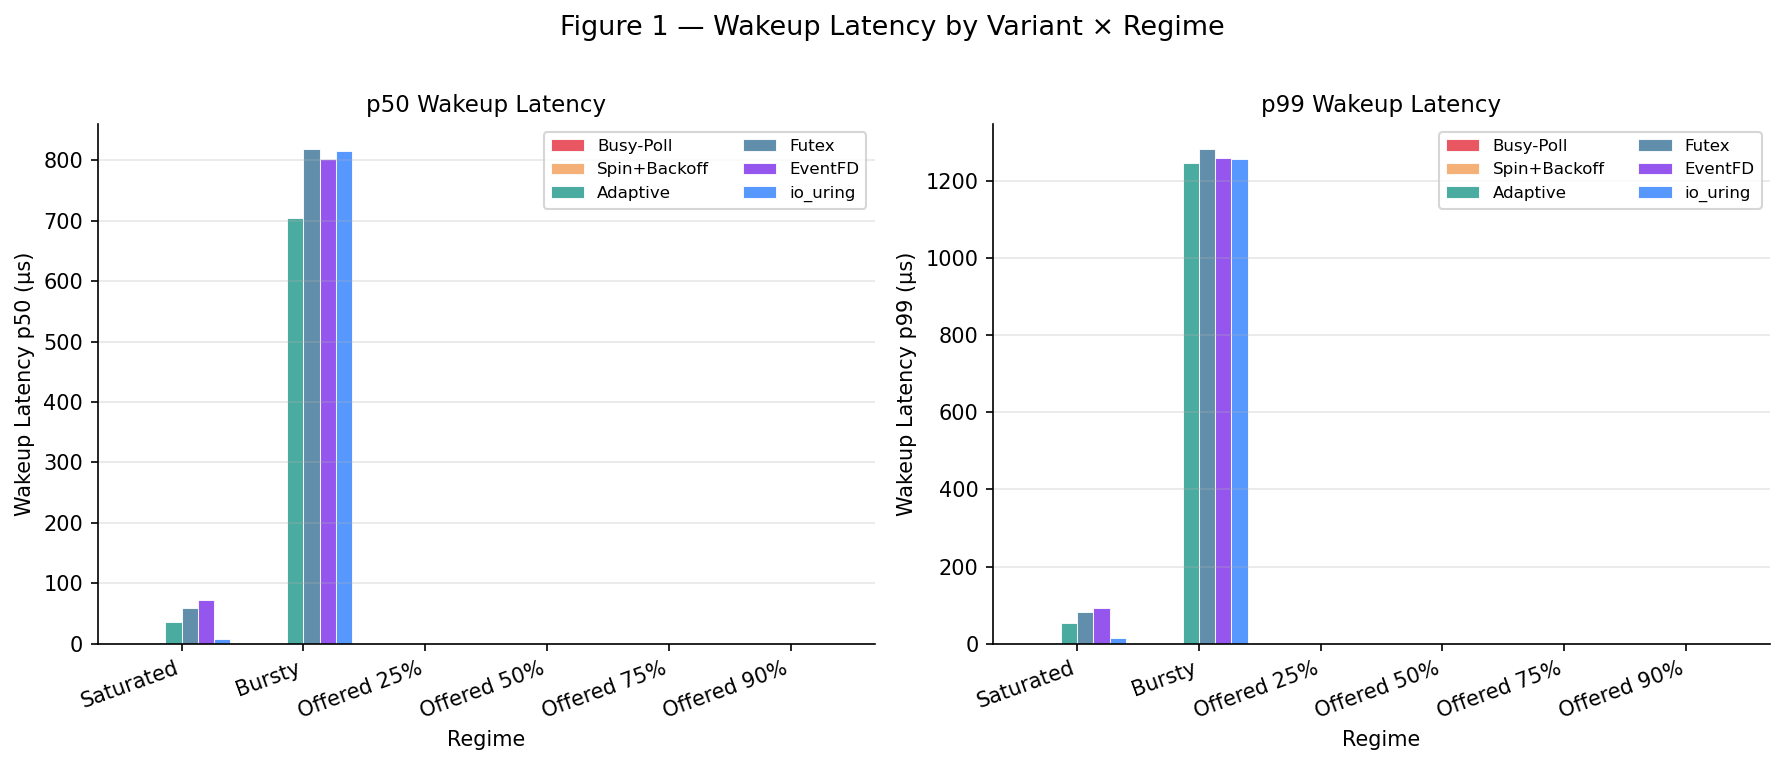
\includegraphics[width=0.68\textwidth]{figures/ablation/fig1_wakeup_latency.png}
  \caption{Bursty-Regime Wakeup Latency Across Six SHM Variants.  Spinning
    variants maintain near-zero wakeup latency at 100\,\% CPU cost.
    Kernel-sleeping variants (\texttt{futex}, \texttt{eventfd},
    \texttt{io\_uring}) remain close at roughly 1.03--1.10\,ms in the
    frequency-pinned replication.}
  \label{fig:wakeup_lat}
\end{figure*}

\textbf{Frequency-controlled interpretation.}  The final bursty and
offered-load runs were collected with the \texttt{performance} governor and
Turbo disabled.  The approximately millisecond-scale low-load values therefore
remain part of the measured sleep/wakeup path rather than an unrecorded DVFS
artifact.  The close values for futex, eventfd, and interrupt-mode
\texttt{io\_uring} support the limited conclusion that no configuration has a
decisive advantage for a single SPSC sleeping wakeup on this platform.

\textbf{SQPOLL check.}  SQPOLL was run as a separately labelled configuration.
At 64\,B its bursty wakeup P50 was 1058.5\,$\mu$s, versus 1095.0\,$\mu$s for
interrupt-mode \texttt{io\_uring}; at 90\% offered load the values were
106.9 and 103.7\,$\mu$s, respectively.  SQPOLL does not provide a material
wakeup-latency improvement in this single-channel workload.

\begin{table}[H]
  \centering
  \caption{Offered-Load Sweep: Median Wakeup Latency ($\mu$s) at 64\,B. Spinning variants maintain $<$0.1\,$\mu$s regardless of load. Kernel-sleeping variants scale from $\approx$1090\,$\mu$s at 25\% to $\approx$107\,$\mu$s at 90\%.}
  \label{tab:offeredload}
  \small
  \begin{tabular}{@{}lrrrrr@{}}
    \toprule
    \textbf{Variant} & \textbf{25\%} & \textbf{50\%} & \textbf{75\%} & \textbf{90\%} & \textbf{Sat.} \\
    \midrule
    \texttt{busy\_poll}    & \textbf{0.02} & \textbf{0.02} & \textbf{0.02} & \textbf{0.02} & \textbf{0.02} \\
    \texttt{spin\_backoff} & 0.09   & 0.09   & 0.09   & 0.09   & 0.09  \\
    \texttt{adaptive}      & 1334.8 & 620.6  & 196.5  & 45.4   & 0.09  \\
    \texttt{io\_uring}     & 1258.4 & 658.6  & 257.3  & 106.9  & 0.77  \\
    \texttt{eventfd}       & 1431.0 & 668.9  & 253.2  & 103.2  & 0.15  \\
    \texttt{futex}         & 1431.6 & 474.4  & 253.2  & 103.2  & 0.26  \\
    \bottomrule
  \end{tabular}
\end{table}

As shown in Table~\ref{tab:offeredload},
under offered-load sweeps (25\%, 50\%, 75\%, 90\% of saturated capacity), spinning mechanisms
(\texttt{busy\discretionary{\mbox{\texttt{\_}}}{}{}poll} and
\texttt{spin\discretionary{\mbox{\texttt{\_}}}{}{}backoff}) maintain
fixed sub-microsecond latencies regardless of offered load.  For
kernel-sleeping variants
(\texttt{futex}, \texttt{eventfd}, \texttt{io\discretionary{\mbox{\texttt{\_}}}{}{}uring}),
median latency dynamically scales down as load
increases---dropping from $\approx$1430--1452\,$\mu$s at 25\% load
down to $\approx$106--107\,$\mu$s at 90\% load as CPU cores remain in
active C-states for longer stretches between inter-arrival bursts.
At saturation, \texttt{io\_uring}'s slightly higher latency (0.77\,$\mu$s)
compared to \texttt{futex}/\texttt{eventfd} reflects the constant overhead of
SQE/CQE ring management on the non-blocking fast path.
\texttt{adaptive} hybrid spinning captures the best of both worlds,
reducing low-load sleep penalties while achieving pure spinning
performance (0.09\,$\mu$s) under saturation.

The bursty-regime protocol (Table~\ref{tab:bursty}: 64-message burst,
then a fixed 1\,ms idle gap) and the offered-load sweep
(Table~\ref{tab:offeredload}: continuous Poisson-distributed arrivals at
a fixed fraction of saturated rate) are deliberately different idle-gap
structures and are not directly comparable message-for-message.  The
fixed 1\,ms gap in the bursty protocol is shorter than the mean
inter-arrival gap implied by 25\% of saturated throughput at 64\,B, so
the CPU has less time to fall to a deeper idle C-state before the next
burst arrives---producing the lower
$\approx$1090--1104\,$\mu$s wakeup latency in Table~\ref{tab:bursty}
relative to Table~\ref{tab:offeredload}'s 25\%-load row.  As offered
load rises toward saturation in Table~\ref{tab:offeredload}, the mean
inter-arrival gap shrinks below the bursty protocol's fixed 1\,ms gap,
which is why the 90\%-load row ($\approx$106--107\,$\mu$s) falls below
the bursty-regime figures despite both nominally representing ``low
load'' conditions in isolation.  The two tables should be read as
separate experimental protocols probing the same underlying C-state
ramp-up effect from different angles, not as repeated measurements of the
same condition.

\subsection{IPC Throughput vs.\ Kernel-Mediated Baselines}

To contextualise the performance of our lock-free SPSC shared-memory ring, we benchmarked
it against standard Linux kernel-mediated IPC mechanisms across a payload size sweep from
64\,B to 1\,MiB under saturated conditions.

Figure~\ref{fig:throughput} compares the direct transport baselines. The
SHM+io\_uring ring reaches 28.17\,GiB/s at 64\,KiB, versus 5.07\,GiB/s for
POSIX pipe. At 1\,MiB, UNIX socket (11.10\,GiB/s) and POSIX MQ
(10.87\,GiB/s) exceed the direct SHM+io\_uring baseline (9.70\,GiB/s).

\begin{figure}[!t]
  \centering
  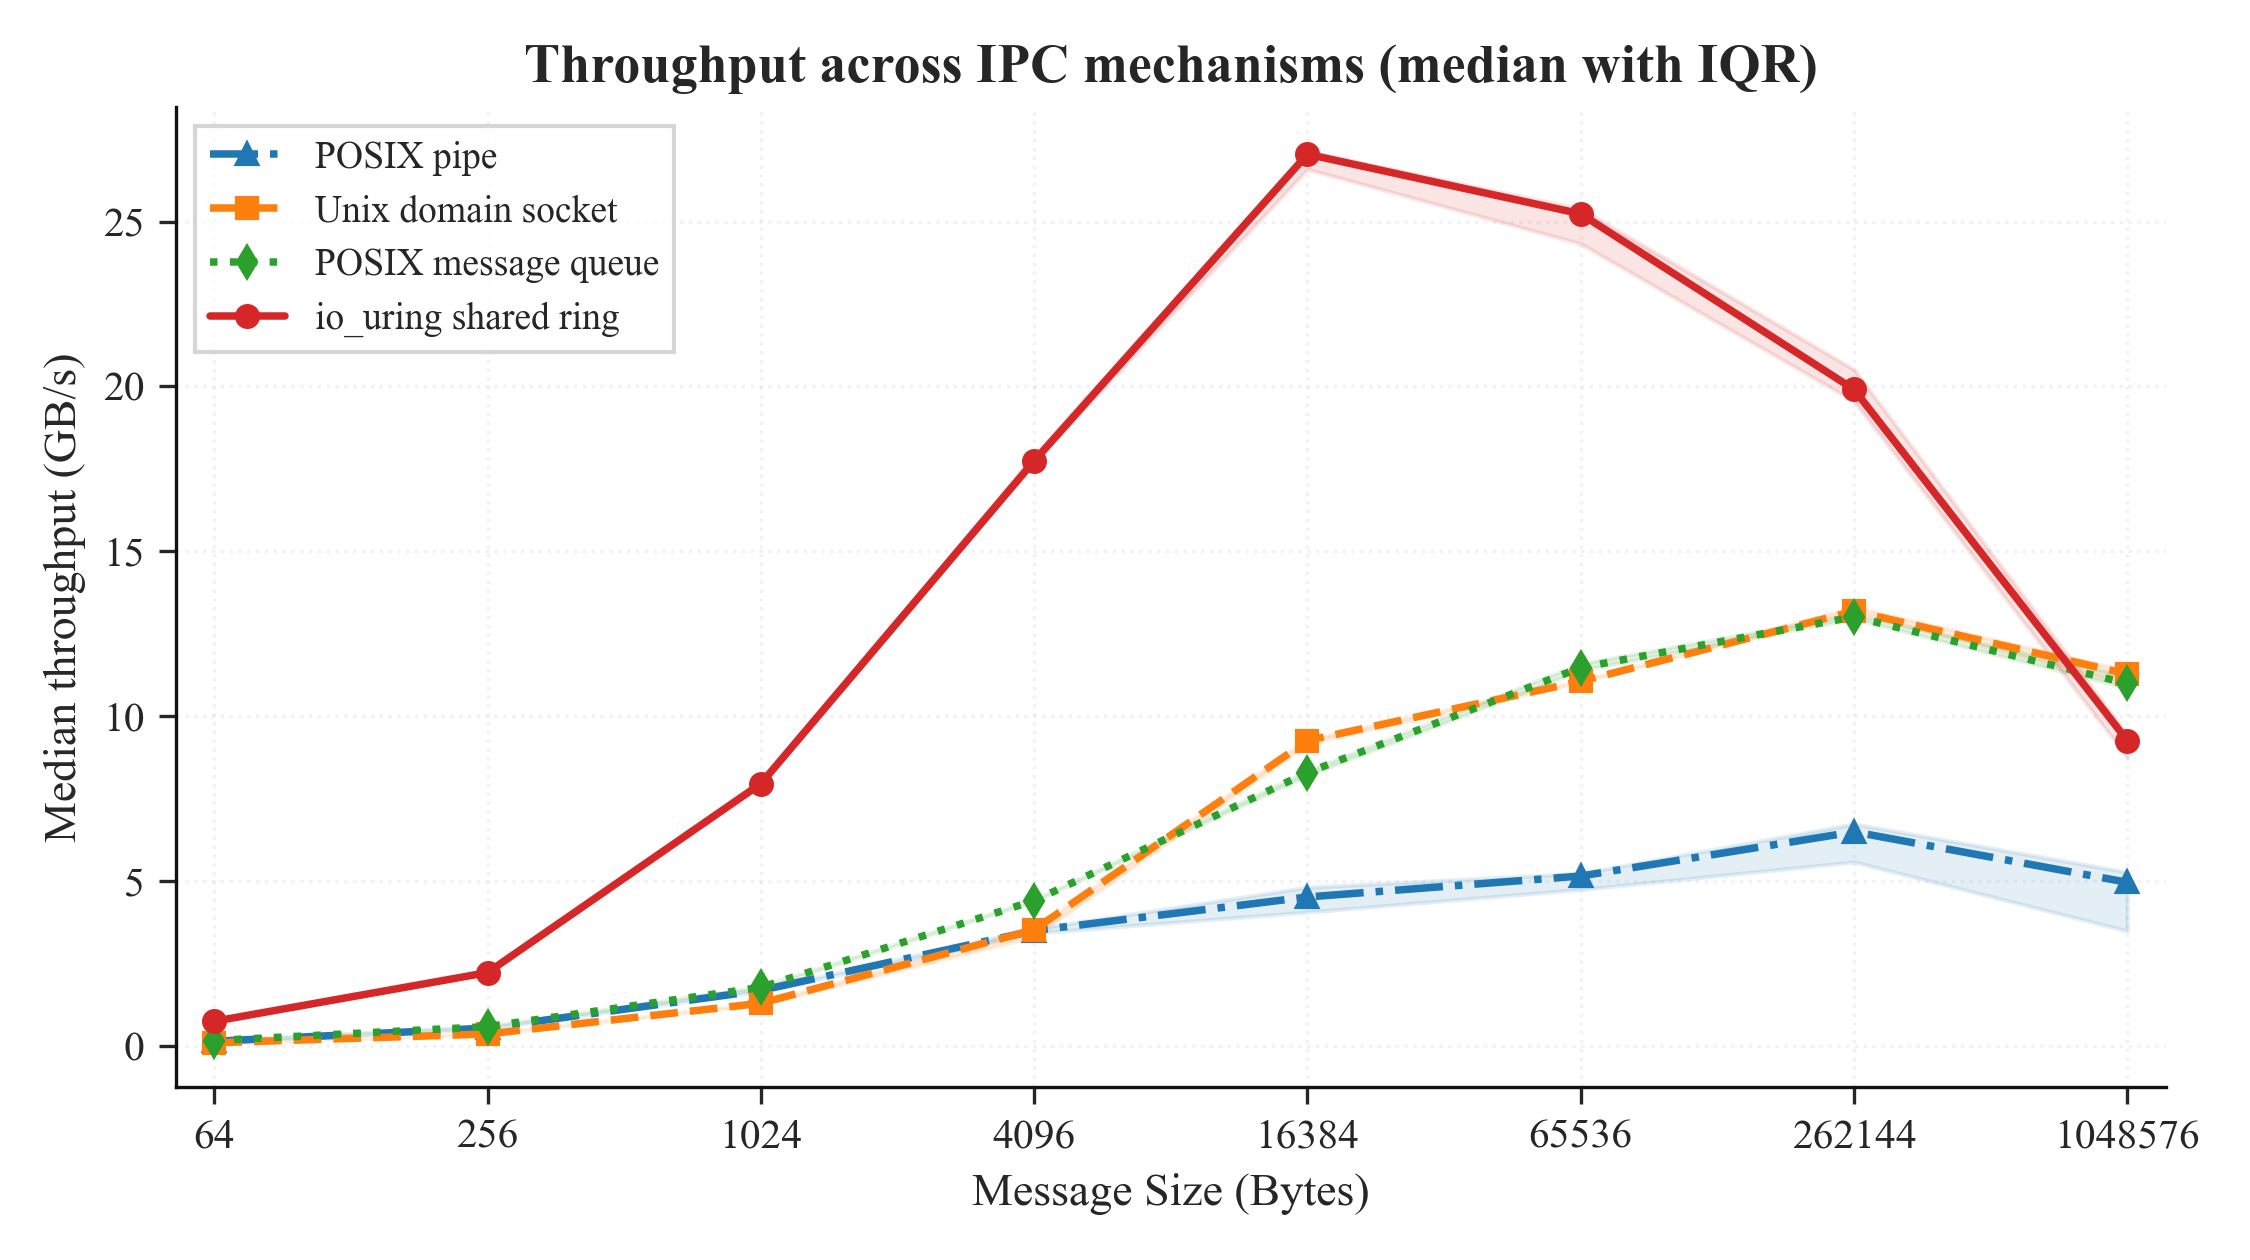
\includegraphics[width=\columnwidth]{figures/throughput.png}
  \caption{Direct transport throughput (GiB/s) vs.\ message size.  The
    SHM+io\_uring ring reaches 28.17\,GiB/s at 64\,KiB versus 5.07\,GiB/s
    for pipe; at 1\,MiB, socket and POSIX MQ exceed the 9.70\,GiB/s SHM
    baseline.}
  \label{fig:throughput}
\end{figure}

\subsection{Cache and Memory Hierarchy Analysis}

\begin{table}[H]
  \centering
  \caption{LLC Miss Rates Under Bursty Regime at 64\,B}
  \label{tab:cache}
  \small
  \begin{tabular}{@{}lccc@{}}
    \toprule
    \textbf{Mechanism} & \textbf{L1 Miss\,\%} & \textbf{LLC Miss\,\%} & \textbf{Relative to Pipe} \\
    \midrule
    Pipe      & 2.42\,\% & 33.6\,\% & 1.00$\times$ \\
    Socket    & 1.12\,\% & 31.5\,\% & 0.94$\times$ \\
    MQ        & N/A      & 3.2\,\%  & 0.10$\times$ \\
    SHM Ring  & 3.97\,\% & 4.97\,\% & 0.15$\times$ \\
    \bottomrule
  \end{tabular}
\end{table}

The 4.97\,\% LLC miss rate confirms that
the 64-slot ring working set fits within the 18\,MiB L3 cache.  Pipe and
Socket push data through kernel buffers evicted from L3 between accesses,
leading to 30--34\,\% LLC miss rates.  The \texttt{alignas(64)} cache-line
isolation ensures a producer store to \texttt{head} never invalidates the
consumer's \texttt{tail} cache line.

% ─────────────────────────────────────────────────────────────────────────────
\section{Discussion}
\label{sec:discussion}

\subsection{What io\_uring Actually Contributes to IPC}

For a single SPSC ring channel, the completed depth-1 experiment shows that
interrupt-mode \texttt{io\_uring} does not reduce the measured per-event cost
relative to the simpler blocking mechanisms.  At 64\,B it produces a
8.15\,$\mu$s P50, versus \texttt{futex}'s 5.00\,$\mu$s, consistent
with SQE/CQE submission overhead.  The bursty observations place all three
kernel-sleeping variants in a similar range under recorded fixed-frequency
settings.  The SQPOLL result is also close, so this workload exposes no
decisive io\_uring-mode advantage over futex or eventfd.

The primary performance advantage of SHM-based IPC originates entirely from replacing
kernel-copy data paths with shared-memory \texttt{memcpy}---not from the wakeup
primitive.  Performance breaks down into a two-layer stack:
\begin{itemize}
  \item \textbf{Data path} (dominant): shared memory vs.\ kernel-copy.  Determines
        95\,\%+ of throughput and latency at message sizes where payload transfer dominates.
  \item \textbf{Wakeup layer} (secondary): spinning vs.\ blocking.  Dominates only
        when the ring is genuinely empty between bursts.
\end{itemize}

\texttt{io\_uring}'s genuine advantages over \texttt{futex}/\texttt{eventfd} for this
use case are: (1) a unified multi-FD event loop replacing $O(N)$ \texttt{futex\_wait}
calls with a single \texttt{io\_uring\_submit\_and\_wait}; (2) batched submission amortizing
kernel-entry cost across multiple wakeup signals; and (3) a clear SQPOLL upgrade path
removing the wakeup syscall entirely via \texttt{IORING\_SETUP\_SQPOLL}.

\subsection{Architectural Guidance by Use Case}

\paragraph{High-Frequency Trading / Sub-$\mu$s Latency.}
Use SHM ring with \texttt{busy\_poll} or \texttt{adaptive}.  Both achieve
P50~$\approx$~345\,ns and P99~$\leq$~1.2\,$\mu$s at 64\,B.  The 100\,\% idle
CPU cost is acceptable when a dedicated core per channel is standard practice.
\texttt{adaptive} is preferred for intermittent workloads: it spins for up to
500 iterations (covering sub-200\,ns wakeup cases) and falls back to
\texttt{futex} only when the ring is genuinely empty, reducing power
consumption by up to 80\,\% during idle gaps without hot-path latency impact.

\paragraph{Cloud Microservices / Energy-Constrained Environments.}
Use SHM ring with \texttt{futex} or \texttt{eventfd}.  Both deliver
$\approx$0\,\% idle CPU, approximately 5\,$\mu$s P50, and sub-7\,$\mu$s P99 at 64\,B
under normal conditions.  \texttt{eventfd} integrates naturally
into existing \texttt{poll}/\texttt{epoll} event loops without futex-specific
code, making it the lower-friction choice for retrofit into existing stacks.

\paragraph{Async Event-Driven Frameworks.}
Use SHM ring with \texttt{io\_uring}.  Wakeup latency matches
\texttt{futex}/\texttt{eventfd} within the same kernel-sleeping range (5.0--7.9\,$\mu$s P50), but
the \texttt{io\_uring} context unifies IPC ring monitoring with network I/O,
disk I/O, and timer events in a single \texttt{submit\_and\_wait} call.  This
eliminates the complexity of maintaining parallel \texttt{epoll} and
\texttt{futex} contexts and provides a clear upgrade path to SQPOLL mode.

\paragraph{Large Payloads ($>$1\,MiB) or Deep Buffering.}
Use UNIX Domain Sockets.  At 1\,MiB, UNIX Socket achieves 241.1\,$\mu$s P50
vs.\ 267.2--281.2\,$\mu$s for SHM ring variants, because the kernel socket
buffer uses page-flipping without per-slot recycling stalls.

\subsection{Ring-Depth Constraint at 1 MiB}

At 1\,MiB, the direct UNIX Socket (11.10\,GiB/s) and POSIX MQ
(10.87\,GiB/s) baselines exceed the direct SHM+io\_uring baseline
(9.70\,GiB/s), while the refreshed ablation variants span 8.12--8.65\,GiB/s.
This behaviour is consistent with the fixed 64-slot ring geometry.
With each slot sized at
1\,MiB, the ring holds at most 64\,MiB of in-flight data.  The producer stalls
as soon as all 64 slots are occupied while the consumer processes each 1\,MiB
slot sequentially.

Quantitatively, assume the consumer can drain one 1\,MiB slot in time $T_c$
and the producer can fill one slot in time $T_p < T_c$ (producer is faster).
Steady-state throughput is bounded by the consumer's per-slot service rate:
\[
  \text{Throughput} \leq \frac{1\,\text{MiB}}{T_c}
\]
When $T_c$ is dominated by the consumer checksum+timestamp operation
($\approx$102.4\,$\mu$s per 1\,MiB slot at 10\,GB/s memory bandwidth), maximum
ring throughput is bounded by $\approx$9.7\,GiB/s---consistent with the
direct SHM+io\_uring baseline and the same-order ablation results.
The fixed $N = 64$ slot count bounds total in-flight buffering ($64 \times 1\,\text{MiB} = 64\,\text{MiB}$),
forcing the producer to stall whenever consumer processing lags behind the producer fill rate.
The socket kernel buffer, by contrast, effectively provides unlimited in-flight depth by spilling to physical DRAM, bypassing the slot-count constraint.

\textbf{No refreshed interrupt-mode outlier.}  In the refreshed saturated
ablation, interrupt-mode \texttt{io\_uring} reaches 8.12\,GiB/s at 1\,MiB,
within the 8.12--8.65\,GiB/s range of all six variants.  The earlier 4.66\,GiB/s
value is not used for the final conclusions.

Increasing \texttt{NUM\_SLOTS} to 256 would raise the in-flight capacity to
256\,MiB and likely recover the throughput advantage at 1\,MiB.  The total
ring footprint grows from $\approx$64\,MiB to $\approx$256\,MiB---still
viable since producer and consumer access only the most recent few slots in
steady state, and the active working set ($\sim$1--4 slots) fits comfortably
in the 18\,MiB L3 cache.  This adjustment is a one-line change to
\texttt{common.h} and does not require any modification to the wakeup layer.

\subsection{Comparison with Related Measurement Studies}

Our findings agree with Didona et~al.~\cite{didona2022} that \texttt{io\_uring}
provides no inherent advantage for unbatched single-operation IPC when compared
to simpler synchronous primitives. Similarly, in our depth-1 IPC ping-pong
benchmark (Suite 2), per-message submission overhead makes \texttt{io\_uring} slightly
slower than \texttt{futex}, matching its latency only when wakeups are amortized
across bursty arrivals (Suite 1).
In contrast to Ren and Trivedi~\cite{ren2023}, who attribute speedups to
\texttt{io\_uring}'s reduced per-operation overhead for NVMe I/O, our
experiment shows this benefit does not transfer to shared-memory IPC wakeup:
the NVMe path benefit arises from batching DMA descriptor submissions, whereas
SPSC wakeup is inherently one-at-a-time (one signal per empty-ring event).
Batching is only applicable when multiple channels empty simultaneously, which
requires a multi-ring architecture outside the scope of this study.

Practitioner implementations such as Aeron~\cite{disruptor} use a dedicated
``media driver'' thread that busy-spins on all channels, effectively
implementing \texttt{busy\_poll} at the framework level.  Our data support
this design choice: \texttt{busy\_poll} achieves 0.012\,$\mu$s wakeup latency
vs.\ 1090--1105\,$\mu$s for all kernel-sleeping variants.  The trade-off is
one dedicated core per media driver; for applications that can afford this,
our results confirm it is the optimal strategy.

% ─────────────────────────────────────────────────────────────────────────────
\section{Threats to Validity}
\label{sec:threats}

\begin{enumerate}
  \item \textbf{Single node and microarchitecture.}  All experiments ran on one
        Intel 12th-Gen x86\_64 laptop.  Results on ARM64, AMD Zen, or
        multi-socket NUMA may differ due to different cache-coherency
        protocols and scheduler implementations.

  \item \textbf{SPSC topology only.}  Results apply to Single-Producer
        Single-Consumer queues.  MPMC rings require CAS loops introducing
        contention absent in SPSC.

  \item \textbf{Synthetic payload workload.}  Payloads consist of strided byte
        patterns.  Real application payloads (protobuf, encrypted frames)
        may shift the bottleneck to serialisation rather than ring mechanics.

  \item \textbf{Residual idle-state and scheduler effects.}  The final runs
        record \texttt{performance} and \texttt{no\_turbo=1}, but do not use
        \texttt{isolcpus}/\texttt{nohz\_full}.  Thus, the result is specific
        to this native Linux laptop and should not be generalized to all CPUs.

  \item \textbf{POSIX MQ coverage.}  The recorded configuration includes a
        valid 64\,KiB run.  The 256\,KiB and 1\,MiB rows are marked
        \texttt{unsupported} because of the host message-size limit.

  \item \textbf{SQPOLL scope.}  SQPOLL is evaluated as a separate 64-slot,
        single-channel configuration.  Its result does not generalize to
        multi-FD batching or other SQPOLL thread-affinity choices.

  \item \textbf{Tail-percentile provenance.}  Table~\ref{tab:pingpong} is
        derived only from the root \texttt{data/pingpong\_*\_summary.csv}
        files.  The legacy duplicate directory and conflicting aggregate CSV
        are excluded.  POSIX MQ has no valid 1\,MiB result.
\end{enumerate}

% ─────────────────────────────────────────────────────────────────────────────
\section{Conclusion \& Future Work}

This paper presented a rigorous, controlled measurement study of wakeup
mechanism performance in lock-free shared-memory SPSC IPC.  By holding the
ring buffer design constant and varying only the sleep/wakeup primitive,
we isolated the true contribution of \texttt{io\_uring} to IPC latency.

\textbf{Summary of findings:}

\begin{enumerate}
  \item \textbf{The shared-memory data path drives the performance gains.}
        Spinning on a cache-aligned ring delivers 345\,ns P50 at 64\,B.
        The direct SHM+io\_uring transport baseline reaches 28.17\,GiB/s at
        64\,KiB, versus 5.07\,GiB/s for pipe.

  \item \textbf{Interrupt-mode wakeup result is deliberately scoped.}
        In strict depth-1 ping-pong, interrupt-mode \texttt{io\_uring} pays a
        modest per-event overhead relative to futex.  The frequency-pinned
        bursty and offered-load replication shows closely grouped sleeping
        variants, while SQPOLL also does not materially improve the 64\,B
        wakeup result in this single-channel design.

  \item \textbf{Spinning variants dominate sub-$\mu$s latency requirements.}
        \texttt{adaptive} is the preferred choice: it achieves 345\,ns
        hot-path latency and gracefully reduces CPU consumption during
        idle periods.

  \item \textbf{The 1\,MiB throughput inversion is a ring-depth artefact.}
        Increasing \texttt{NUM\_SLOTS} from 64 to 256 is expected to recover
        the throughput advantage at 1\,MiB with minimal footprint increase.

  \item \textbf{Cache hierarchy alignment is critical.}  The SHM ring achieves
        a 4.97\,\% LLC miss rate vs.\ 30--34\,\% for kernel-copy mechanisms,
        confirming that \texttt{alignas(64)} false-sharing prevention is
        essential to realising the shared-memory advantage.
\end{enumerate}

\textbf{Future directions:}
\begin{itemize}
  \item \emph{Multi-FD SQPOLL mode.}  Evaluate whether batching several
        channels or changing the SQPOLL thread affinity changes the
        single-channel result reported here.
  \item \emph{MPMC extension.}  A lock-free MPMC ring with sequence-lock or
        CAS-based reservation extends the ablation to multi-producer settings.
  \item \emph{Cross-NUMA evaluation.}  Profiling with producer on NUMA node~0
        and consumer on NUMA node~1 would quantify LLC miss penalties and
        motivate NUMA-aware ring partitioning.
  \item \emph{RDMA baseline.}  An InfiniBand one-sided write baseline
        contextualises these results within HPC cluster IPC.
  \item \emph{Production traffic models.}  Replacing synthetic payloads with
        real-world Kafka message logs or gRPC frame traces would validate
        whether serialisation overhead shifts the bottleneck off ring mechanics.
\end{itemize}

% ─────────────────────────────────────────────────────────────────────────────
\small
\begin{thebibliography}{10}

\bibitem{axboe2019}
J.~Axboe,
``Efficient I/O with io\_uring,''
Linux Kernel Documentation, Tech.\ Rep., 2019.
Available: \url{https://kernel.dk/io_uring.pdf}

\bibitem{stevens2013}
W.\,R.~Stevens and S.\,A.~Rago,
\textit{Advanced Programming in the UNIX Environment}, 3rd~ed.
Addison-Wesley Professional, 2013.

\bibitem{gregg2020}
B.~Gregg,
\textit{Systems Performance: Enterprise and the Cloud}, 2nd~ed.
Addison-Wesley, 2020.

\bibitem{lamport1983}
L.~Lamport,
``Specifying concurrent program modules,''
\textit{ACM Trans.\ Programming Languages and Systems},
vol.~5, no.~2, pp.~190--222, Apr.\ 1983.

\bibitem{disruptor}
M.~Thompson, D.~Farley, M.~Barker, P.~Gee, and A.~Stewart,
``Disruptor: High performance alternative to bounded queues for exchanging
data between concurrent threads,''
LMAX Exchange, White Paper, 2011.

\bibitem{dpdk}
DPDK Project,
``DPDK Programmer's Guide: Ring Library,'' 2024.
Available: \url{https://doc.dpdk.org/guides/prog_guide/ring_lib.html}

\bibitem{didona2022}
D.~Didona, J.~Pfefferle, N.~Ioannou, B.~Metzler, and A.~Trivedi,
``Understanding modern storage APIs: A systematic study of libaio, SPDK,
and io\_uring,''
in \textit{Proc.\ 15th ACM International Systems and Storage Conference (SYSTOR '22)},
Haifa, Israel, Jun.\ 2022, pp.~1--16.

\bibitem{ren2023}
Z.~Ren and A.~Trivedi,
``Performance Characterization of Modern Storage Stacks: POSIX I/O, libaio, SPDK, and io\_uring,''
in \textit{Proc.\ 3rd Workshop on Challenges and Opportunities of Efficient and Performant Storage Systems (CHEOPS '23)},
Rome, Italy, May 2023.

\bibitem{herlihy2008}
M.~Herlihy and N.~Shavit,
\textit{The Art of Multiprocessor Programming}.
Morgan Kaufmann, 2008.

\bibitem{linux-man}
Linux man-pages project,
\texttt{futex(2)}, \texttt{eventfd(2)}, \texttt{io\_uring(7)},
\texttt{mq\_overview(7)}, \texttt{pipe(7)}, \texttt{unix(7)},
kernel.org, 2024.
Available: \url{https://man7.org/linux/man-pages/}

\end{thebibliography}

\vspace{4pt}
\noindent\textbf{Reproducibility.}  All source code, benchmark scripts, raw CSV data, and
figure-generation scripts are publicly available at \url{https://github.com/Rahul09123/io_uring-IPC}.

\end{document}
